\documentclass[9pt,xcolor={svgnames},hyperref={colorlinks,urlcolor=DarkBlue}]{beamer}
\usepackage[colorlinks]{hyperref}
\usepackage{tikz}
\usepackage{pdfpages}
\usepackage{framed}
\usepackage{fancyvrb}
%\usepackage{listings}
\usepackage{verbatim}

\usepackage{minted}
\usepackage{lmodern}
\usepackage{amssymb,amsmath,amscd}
\usepackage{longtable}
\usepackage{booktabs}
\usepackage{graphicx}
\usepackage{fixltx2e}
\usepackage[utf8]{inputenc}
\usepackage{microtype}
\usepackage{marvosym}
\usepackage{parskip}
\usepackage{etoolbox}
\usepackage{algorithm2e}
\usetikzlibrary{tikzmark,chains}
\usepackage{tkz-euclide}
\usetikzlibrary{arrows,%
                petri,%
                topaths,calc,
                automata,shapes.geometric,positioning}%


\usepackage{pgffor}

\graphicspath{ {./pic/}}
\UseMicrotypeSet[protrusion]{basicmath} % disable protrusion for tt fonts
\setlength{\emergencystretch}{3em}  % prevent overfull lines
\providecommand{\tightlist}{\setlength{\itemsep}{0pt}\setlength{\parskip}{0pt}}
\setcounter{secnumdepth}{0}


\definecolor{mintedbg}{rgb}{0.85,0.85,0.85}
\newminted{text}{fontsize=\footnotesize,bgcolor=mintedbg,style=bw, autogobble}
\newminted{c}{fontsize=\footnotesize,bgcolor=mintedbg,style=bw, autogobble}
\newminted{cpp}{fontsize=\footnotesize,bgcolor=mintedbg,style=bw, autogobble}
\newminted{python}{fontsize=\footnotesize,bgcolor=mintedbg,style=bw, autogobble}
\newminted{julia}{fontsize=\footnotesize,bgcolor=mintedbg,style=bw, autogobble}
\newminted{bash}{fontsize=\footnotesize,bgcolor=mintedbg,style=bw, autogobble}
\newminted{cmake}{fontsize=\footnotesize,bgcolor=mintedbg,style=bw, autogobble}


\AtBeginEnvironment{minted}{\let\itshape\relax}


\newcommand{\bb}[1]{\mathbb #1}
\newcommand{\ca}[1]{\mathcal #1}
\newcommand{\RR}{\bb{R}}
\newcommand{\DD}{\bb{D}}
\newcommand{\QQ}{\bb{Q}}
\newcommand{\ZZ}{\bb{Z}}
\newcommand{\NN}{\bb{N}}
\newcommand{\PP}{\bb{P}}
\newcommand{\VV}{\bb{V}}
\newcommand{\CC}{\bb{C}}
\newcommand{\CK}{\ca{K}}
\newcommand{\CN}{\ca{N}}
\newcommand{\CG}{\ca{G}}
\newcommand{\CT}{\ca{T}}
\newcommand{\CI}{\ca{I}}

\newcommand{\vvec}[1]{\vec{#1}}
\newcommand{\vx}{\vvec{x}}
\newcommand{\vy}{\vvec{y}}
\newcommand{\vz}{\vvec{z}}
\newcommand{\vu}{\vvec{u}}
\newcommand{\vv}{\vvec{v}}
\newcommand{\vj}{\vvec{j}}
\newcommand{\vp}{\vvec{p}}
\newcommand{\vq}{\vvec{q}}
\newcommand{\va}{\vvec{a}}
\newcommand{\ve}{\vvec{e}}
\newcommand{\vb}{\vvec{b}}
\newcommand{\vc}{\vvec{c}}
\newcommand{\vd}{\vvec{d}}
\newcommand{\vn}{\vvec{n}}
\newcommand{\vnu}{\vvec{\nu}}
\newcommand{\vnabla}{\vvec{\nabla}}
\newcommand{\vlambda}{\vvec{\lambda}}
\newcommand{\vsigma}{\vvec{\sigma}}

\newcommand{\grad}{\vnabla}
\renewcommand{\div}{\nabla\cdot}


\newcommand{\norm}[1]{\lVert#1\rVert}
\newcommand{\normli}[1]{\lVert#1\rVert_{L^1}}
\newcommand{\normlii}[1]{\lVert#1\rVert_{L^2}}
\DeclareMathOperator{\tr}{tr}
\DeclareMathOperator{\sspan}{span}
\DeclareMathOperator{\supp}{supp}
\DeclareMathOperator{\card}{card}

%%%%%%%%%%%%%%%%%%%%%%%%%%%%%%%%%%%%%%%%%%%%%%%%%%%

% see https://tex.stackexchange.com/questions/46711/reusing-slides-from-beamer-presentations

\newcommand{\DefineSection}[2]{\setbeamertemplate{slide #1}{{#2}}}

\newcommand{\UseSection}[1]{
  \ifbeamertemplateempty{slide #1}%
  {
    \errmessage empty section: {#1}
  }%
  {
    % \opt{texdebug}{\message{        *** Using section: (#1) }}
    \usebeamertemplate{slide #1}%
  }%
}

\newif\iflectureI\lectureIfalse
\newif\iflectureII\lectureIIfalse
\newif\iflectureIII\lectureIIIfalse
\newif\iflectureIV\lectureIVfalse
\newif\iflectureV\lectureVfalse
\newif\iflectureVI\lectureVIfalse
\newif\iflectureVII\lectureVIIfalse
\newif\iflectureVIII\lectureVIIIfalse
\newif\iflectureIX\lectureIXfalse
\newif\iflectureX\lectureXfalse
\newif\iflectureXI\lectureXIfalse
\newif\iflectureXII\lectureXIIfalse
\newif\iflectureXIII\lectureXIIIfalse
\newif\iflectureXIV\lectureXIVfalse
\newif\iflectureXV\lectureXVfalse
\newif\iflectureXVI\lectureXVIfalse
\newif\iflectureXVII\lectureXVIIfalse
\newif\iflectureXVIII\lectureXVIIIfalse
\newif\iflectureXIX\lectureXIXfalse
\newif\iflectureXX\lectureXXfalse
\newif\iflectureXXI\lectureXXIfalse
\newif\iflectureXXII\lectureXXIIfalse
\newif\iflectureXXIII\lectureXXIIIfalse
\newif\iflectureXXIV\lectureXXIVfalse
\newif\iflectureXXV\lectureXXVfalse
\newif\iflectureXXVI\lectureXXVIfalse
\newif\iflectureXXVII\lectureXXVIIfalse
\newif\iflectureXXVIII\lectureXXVIIIfalse
\newif\iflectureXXIX\lectureXXIXfalse

\def\@mylecture{0}
\providecommand{\iflecture}[1]{\ifnumequal{\@mylecture}{#1}}
\newcommand{\mylecture}[1]{%
\def\@mylecture{#1}
\iflecture{1}\lectureItrue{}%
\iflecture{2}\lectureIItrue{}%
\iflecture{3}\lectureIIItrue{}%
\iflecture{4}\lectureIVtrue{}%
\iflecture{5}\lectureVtrue{}%
\iflecture{6}\lectureVItrue{}%
\iflecture{7}\lectureVIItrue{}%
\iflecture{8}\lectureVIIItrue{}%
\iflecture{9}\lectureIXtrue{}%
\iflecture{10}\lectureXtrue{}%
\iflecture{11}\lectureXItrue{}%
\iflecture{12}\lectureXIItrue{}%
\iflecture{13}\lectureXIIItrue{}%
\iflecture{14}\lectureXIVtrue{}%
\iflecture{15}\lectureXVtrue{}%
\iflecture{16}\lectureXVItrue{}%
\iflecture{17}\lectureXVIItrue{}%
\iflecture{18}\lectureXVIIItrue{}%
\iflecture{19}\lectureXIXtrue{}%
\iflecture{20}\lectureXXtrue{}%
\iflecture{21}\lectureXXItrue{}%
\iflecture{22}\lectureXXIItrue{}%
\iflecture{23}\lectureXXIIItrue{}%
\iflecture{24}\lectureXXIVtrue{}%
\iflecture{25}\lectureXXVtrue{}%
\iflecture{26}\lectureXXVItrue{}%
\iflecture{27}\lectureXXVIItrue{}%
\iflecture{28}\lectureXXVIIItrue{}%
\iflecture{29}\lectureXXIXtrue{}%
}
\newcommand{\themylecture}{\@mylecture}




\usetheme{Frankfurt}

\renewcommand{\subsection}[1]{~\newline~\vfill\begin{center}{\large\textbf{#1}}\end{center}\vfill~\newline~}
\renewcommand{\section}[1]{~\newline~\vfill\begin{center}{\LARGE\textbf{#1}}\end{center}\vfill~\newline~}

\setbeamertemplate{navigation symbols}{\hspace{1em}\usebeamerfont{footline} Lecture \@mylecture Slide \insertframenumber}

\newcommand{\oldslide}[2]{
{
  \setbeamercolor{background canvas}{bg=}
  \refstepcounter{framenumber}
  \includepdf[pages={#2}, frame=true,noautoscale,scale=0.93]{#1}
}
}



\newcommand{\titleframe}{
\begin{frame}

  \vfill 

  Scientific Computing WS 2020/2021
  \bigskip 

  Lecture \themylecture

  \bigskip
  Jürgen Fuhrmann

  juergen.fuhrmann@wias-berlin.de

  \vfill~  
\end{frame}
}
\mylecture{1}
\begin{document}

\titleframe{}

%%%%%%%%%%%%%%%%%%%%%%%%%%%%%%%%%%%%%%%%%%%%%%%%%%%%%%%%%%%%%%%%%%%%%%%%%%%%%%%
\begin{frame}{Me}
  \begin{itemize}
  \item
    Name: Dr.~Jürgen Fuhrmann (no, not Prof.)
  \item
    Affiliation: Weierstrass Institute for Applied Analysis and
    Stochastics, Berlin (WIAS);\\ Deputy Head, \emph{Numerical Mathematics and Scientific Computing}
  \item
    Contact: \textbf{juergen.fuhrmann@wias-berlin.de}
  \item Course homepage:  \url{https://www.wias-berlin.de/people/fuhrmann/SciComp-WS2021/}
  \item
    Experience/Field of work:
    
    \begin{itemize}
      \tightlist
    \item
      Numerical solution of partial differential equations (PDEs)
    \item
      Development, investigation, implementation of finite volume
      discretizations for nonlinear systems of PDEs
    \item
      Ph.D.~on multigrid methods
    \item
      Applications: electrochemistry, semiconductor physics,
      groundwater\ldots{}
    \item
      Software development:
      
      \begin{itemize}
        \tightlist
      \item
        WIAS code pdelib (\url{http://pdelib.org})
      \item
        Languages: C, C++, Python, Lua, Fortran, Julia 
      \item
        Visualization: OpenGL, VTK
      \end{itemize}
    \end{itemize}
  \end{itemize}
  
\end{frame}
%%%%%%%%%%%%%%%%%%%%%%%%%%%%%%%%%%%%%%%%%%%%%%%%%%%%%%%%%%%%%%%%%%%%%%%%%%%%%%%

%%%%%%%%%%%%%%%%%%%%%%%%%%%%%%%%%%%%%%%%%%%%%%%%%%%%%%%%%%%%%%%%%%%%%%%%%%%%%%%
\begin{frame}{Admin stuff}
  \begin{itemize}
  \item Lectures will be recorded
  \item Slides + Julia notebooks will be available from the course home page
    \url{https://www.wias-berlin.de/people/fuhrmann/SciComp-WS2021/}
  \item Weekly material uploads by Wed night (hopefully)
  \item Official lecture times: Thu 16-18 and Fri 16-18 will be used for
    feedback sessions with zulip chat and zoom. 
  \item Zoom links will be provided in the chat or per email.
  \item I will use the email address used for enrolling for all communication, zulip invitations
    etc. Please keep me informed about any changes.
  \item Please provide missing ``Matrikelnummern''
  \item All code examples and assignments will be in Julia, either as notebooks or
    as Julia files. Things should work on  Linux, MacOSX, Windows
  \item
    Access to examination
    \begin{itemize}
    \item
      Attend \(\approx\) 80\% of lectures
    \item
      Return assignments
    \end{itemize}
  \end{itemize}
  
\end{frame}
%%%%%%%%%%%%%%%%%%%%%%%%%%%%%%%%%%%%%%%%%%%%%%%%%%%%%%%%%%%%%%%%%%%%%%%%%%%%%%%



%%% Local Variables:
%%% mode: latex
%%% TeX-master: "l01-intro"
%%% End:



\begin{frame}
  \section{Introduction}
\end{frame}


\begin{frame}\frametitle{There was a time when ``computers'' were humans}
  
  \begin{minipage}{0.45\textwidth}
    \includegraphics[width=\textwidth]{pic/HarvardComputers.jpg}\newline
    Harvard Computers, circa 1890\newline
    {\tiny By Harvard College Observatory - Public Domain}\newline
    {\tiny \url{https://commons.wikimedia.org/w/index.php?curid=10392913}}
  \end{minipage}\hfill
  \begin{minipage}{0.45\textwidth}
    \includegraphics[width=\textwidth]{pic/harvardobs.jpg}
    \vspace{1.25cm}
    It was about science -- astronomy
  \end{minipage}

  Computations of course have been performed since ancient times. One can 
  trace back the termin ``computer'' applied to humans at least until 1613. 
  \only<article>{
    The reference is R. Brathwaite, The Yong Mans Gleanings, London 2014,
    full text available: \url{https://quod.lib.umich.edu/e/eebo/A00514.0001.001?rgn=main;view=fulltext}
  }

  The ``Harvard computers'' became very famous in this context. Incidently, they were
  mostly female. They predate the NASA human computers of recent movie fame.
  \only<article>{See \url{https://en.wikipedia.org/wiki/Harvard_Computers}}

\end{frame}


\begin{frame}\frametitle{Does this scale ?}
  
  \begin{minipage}{0.45\textwidth}
    \includegraphics[width=\textwidth]{pic/richardsbook}
    \vspace{1.25cm}
    
    L.F.Richardson 1922
  \end{minipage}\hfill
  \begin{minipage}{0.45\textwidth}
    \includegraphics[width=\textwidth]{pic/weatherfactory.jpg}
    
    64000 computers predicting weather (1986 Illustration of L.F. Richardson's vision
    by S. Conlin)
  \end{minipage}
  
  \begin{itemize}
    \tightlist
  \item
    This was about weather, not science in the first place
  \item
    Science \emph{and} Engineering need computing
  \end{itemize}
  
\end{frame}
%%%%%%%%%%%%%%%%%%%%%%%%%%%%%%%%%%%%%%%%%%%%%%%%%%%%%%%%%%%%%%%%%%% 

%%%%%%%%%%%%%%%%%%%%%%%%%%%%%%%%%%%%%%%%%%%%%%%%%%%%%%%%%%%%%%%%%%% 
\begin{frame}\frametitle{Computing was taken over by machines}

  \begin{center}
    \includegraphics[width=0.95\textwidth]{pic/moore.png}
    \vspace{-0.15cm}

    {\tiny By Max Roser - https://ourworldindata.org/uploads/2019/05/Transistor-Count-over-time-to-2018.png, CC BY-SA 4.0, https://commons.wikimedia.org/w/index.php?curid=79751151}
  \end{center}

\end{frame}
%%%%%%%%%%%%%%%%%%%%%%%%%%%%%%%%%%%%%%%%%%%%%%%%%%%%%%%%%%%%%%%%%%% 

%%%%%%%%%%%%%%%%%%%%%%%%%%%%%%%%%%%%%%%%%%%%%%%%%%%%%%%%%%%%%%%%%%% 
\begin{frame}\frametitle{Computational engineering}

  \begin{itemize}
  \item
    Starting points: Nuclear weapons + rocket design, ballistic
    trajectories, weather \ldots{}
  \item
    Now ubiquitous:

    \begin{itemize}
      \tightlist
    \item
      Structural engineering
    \item
      Car industry
    \item
      Oil recovery
    \item
      Semiconductor design
    \item
      \ldots{}
    \end{itemize}
  \item
    Use of well established, verfied, well supported commercial codes

    \begin{itemize}
      \tightlist
    \item
      Comsol
    \item
      ANSYS
    \item
      Eclipse
    \item
      \ldots{}
    \end{itemize}
  \end{itemize}

\end{frame}
%%%%%%%%%%%%%%%%%%%%%%%%%%%%%%%%%%%%%%%%%%%%%%%%%%%%%%%%%%%%%%%%%%% 

%%%%%%%%%%%%%%%%%%%%%%%%%%%%%%%%%%%%%%%%%%%%%%%%%%%%%%%%%%%%%%%%%%% 
\begin{frame}\frametitle{As soon as computing machines became available \ldots{}}

  \ldots{} Scientists ``misused'' them to satisfy their curiosity

  \begin{minipage}{0.35\textwidth}
    \includegraphics[width=\textwidth]{pic/fpupic}
  \end{minipage}\hfill
  \begin{minipage}{0.6\textwidth}
    \includegraphics[width=\textwidth]{pic/fputitle}
  \end{minipage}


  ``\ldots{} Fermi became interested in the development and potentialities
  of the electronic computing machines. He held many discussions
  {[}\ldots{}{]} of the kind of future problems which could be studied
  through the use of such machines.''

  Fermi,Pasta and Ulam studied particle systems with \emph{nonlinear}
  interactions

  Calculations were done on the MANIAC-1 computer at Los Alamos

\end{frame}
%%%%%%%%%%%%%%%%%%%%%%%%%%%%%%%%%%%%%%%%%%%%%%%%%%%%%%%%%%%%%%%%%%% 

%%%%%%%%%%%%%%%%%%%%%%%%%%%%%%%%%%%%%%%%%%%%%%%%%%%%%%%%%%%%%%%%%%% 
\begin{frame}\frametitle{And they still do\ldots{}}

  \begin{minipage}{0.45\textwidth}
    \includegraphics[width=\textwidth]{pic/ligo20160211a.jpg}
    
    
    {\tiny Caltech/MIT/LIGO Lab }
  \end{minipage}\hfill
  \begin{minipage}{0.45\textwidth}
    \includegraphics[width=\textwidth]{pic/ligo20160211d.jpg}
    
    
    {\tiny SXS, the Simulating eXtreme Spacetimes (SXS) project (\url{http://www.black-holes.org})}
  \end{minipage}
  
  Verification of the detection of gravitational waves by numerical
  solution of Einstein's equations of general relativity using the
  ``Spectral Einstein Code''

  Computations significantly contributed to the 2017 Nobel prize in physics
\end{frame}
%%%%%%%%%%%%%%%%%%%%%%%%%%%%%%%%%%%%%%%%%%%%%%%%%%%%%%%%%%%%%%%%%%% 

%%%%%%%%%%%%%%%%%%%%%%%%%%%%%%%%%%%%%%%%%%%%%%%%%%%%%%%%%%%%%%%%%%% 
\begin{frame}\frametitle{Scientific computing}

  \textbf{``The purpose of computing is insight, not numbers.''}\\
  (\url{https://en.wikiquote.org/wiki/Richard_Hamming})

  \begin{itemize}
    \tightlist
  \item
    Frontiers of Scientific Computing

    \begin{itemize}
      \tightlist
    \item
      Insight into complicated phenomena not accessible by other methods
    \item
      Improvement of models to better fit reality
    \item
      Improvment of computational methods
    \item
      Generate testable hypothesis
    \item
      Support experimentation in other scientific fields
    \item
      Exploration of new computing capabilities
    \item
      Prediction, optimization of complex systems
    \end{itemize}
  \item
    Good scientifc practice

    \begin{itemize}
      \tightlist
    \item
      Reproducibility
    \item
      Sharing of ideas and knowledge
    \end{itemize}
  \item
    Interdisciplinarity

    \begin{itemize}
      \tightlist
    \item
      Numerical Analysis
    \item
      Computer science
    \item
      Modeling in specific fields
    \end{itemize}
  \end{itemize}

\end{frame}
%%%%%%%%%%%%%%%%%%%%%%%%%%%%%%%%%%%%%%%%%%%%%%%%%%%%%%%%%%%%%%%%%%% 

%%%%%%%%%%%%%%%%%%%%%%%%%%%%%%%%%%%%%%%%%%%%%%%%%%%%%%%%%%%%%%%%%%% 
\begin{frame}\frametitle{General approach}

  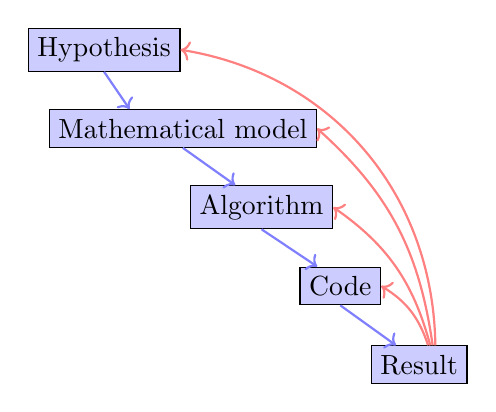
\begin{tikzpicture}
    \node (Hyp) at (2,4) [fill=blue!20,draw] {Hypothesis};
    \node (Mod) at (3,3) [fill=blue!20,draw] {Mathematical model};
    \node (Alg) at (4,2) [fill=blue!20,draw] {Algorithm};
    \node (Cod) at (5,1) [fill=blue!20,draw] {Code};
    \node (Res) at (6,0) [fill=blue!20,draw] {Result};


    \draw[->, blue!50, thick] (Hyp.south) to (Mod.160);
    \draw[->, blue!50, thick] (Mod.south) to (Alg.140);
    \draw[->, blue!50, thick] (Alg.south) to (Cod.140);
    \draw[->, blue!50, thick] (Cod.south) to (Res.140);
    \draw[->, red!50, thick] (Res.65) to[bend right=20] (Cod.east);
    \draw[->, red!50, thick] (Res.60) to[bend right=20] (Alg.east);
    \draw[->, red!50, thick] (Res.55) to[bend right=20] (Mod.east);
    \draw[->, red!50, thick] (Res.50) to[bend right=40] (Hyp.east);
  \end{tikzpicture}

  \begin{itemize}
    \tightlist
  \item
    Possible (probable) involvement of different persons, institutions
  \item
    It is important to keep interdisciplinarity in mind
  \end{itemize}

\end{frame}
%%%%%%%%%%%%%%%%%%%%%%%%%%%%%%%%%%%%%%%%%%%%%%%%%%%%%%%%%%%%%%%%%%% 

%%%%%%%%%%%%%%%%%%%%%%%%%%%%%%%%%%%%%%%%%%%%%%%%%%%%%%%%%%%%%%%%%%% 
\begin{frame}\frametitle{Scientific computing tools}

  Many of them are Open Source

  \begin{itemize}
    \tightlist
  \item
    General purpose environments

    \begin{itemize}
      \tightlist
    \item
      Matlab
    \item
      COMSOL
    \item
      Python + ecosystem
    \item
      R + ecosystem
    \item
      \textbf{Julia}
    \end{itemize}
  \item
    ``Classical'' computer languages + compilers

    \begin{itemize}
      \tightlist
    \item
      Fortran
    \item
      C, C++
    \end{itemize}
  \item
    Established special purpose libraries

    \begin{itemize}
      \tightlist
    \item
      Linear algebra: LAPACK, BLAS, UMFPACK, Pardiso
    \item
      Mesh generation: \textbf{triangle}, TetGen, NetGen
    \item
      Eigenvalue problems: ARPACK
    \item
      Visualization libraries: VTK
    \end{itemize}
  \item
    Tools in the ``background''

    \begin{itemize}
      \tightlist
    \item
      Build systems Make, CMake
    \item
      Editors + IDEs (emacs, jedit, eclipse, atom, Visual Studio Code)
    \item
      Debuggers
    \item
      Version control (svn, \textbf{git}, hg)
    \end{itemize}
  \end{itemize}

\end{frame}

\begin{frame}\frametitle{Confusio Linguarum}

  \begin{minipage}{0.45\textwidth}
    \includegraphics[width=\textwidth]{pic/Babel_1166-12.jpg}
  \end{minipage}\hfill
  \begin{minipage}{0.45\textwidth}
    "And   the  whole   land   was   of  one   language   and  of   one
    speech. ...  And they said, Go to, let us build  us a city and a
    tower whose top may  reach unto heaven. ...  And the Lord said,
    behold,   the   people   is   one,   and   they   have   all   one
    language. ... Go to, let  us go down, and  there confound their
    language that  they may not  understand one another’s  speech.  So
    the Lord  scattered them abroad from  thence upon the face  of all
    the earth." (Daniel 1:1-7)
  \end{minipage}

\end{frame}
%%%%%%%%%%%%%%%%%%%%%%%%%%%%%%%%%%%%%%%%%%%%%%%%%%%%%%%%%%%%%%%%%%% 

%%%%%%%%%%%%%%%%%%%%%%%%%%%%%%%%%%%%%%%%%%%%%%%%%%%%%%%%%%%%%%%%%%% 
\begin{frame}\frametitle{Once again Hamming}

  \ldots{}of ``Hamming code'' and ``Hamming distance'' fame, who started
  his carrier programming in Los Alamos:

  ``Indeed, one of my major complaints about the computer field is that
  whereas Newton could say,''If I have seen a little farther than others,
  it is because I have stood on the shoulders of giants," I am forced to
  say, ``Today we stand on each other's feet.'' Perhaps the central
  problem we face in all of computer science is how we are to get to the
  situation where we build on top of the work of others rather than
  redoing so much of it in a trivially different way. Science is supposed
  to be cumulative, not almost endless duplication of the same kind of
  things." (1968)

  \begin{itemize}
    \tightlist
  \item
    2017 this is still a problem
  \end{itemize}

\end{frame}
%%%%%%%%%%%%%%%%%%%%%%%%%%%%%%%%%%%%%%%%%%%%%%%%%%%%%%%%%%%%%%%%%%% 

%%%%%%%%%%%%%%%%%%%%%%%%%%%%%%%%%%%%%%%%%%%%%%%%%%%%%%%%%%%%%%%%%%% 
\begin{frame}\frametitle{Intended  aims  and topics of this course}

  \begin{itemize}
  \item
    Indicate a reasonable path within this labyrinth
  \item
    Introduction to  Julia
  \item
    Software management skills (version control)
  \item
    Relevant topics from numerical analysis
  \item
    Focus on partial differential equation (PDE) solution
    \begin{itemize}
      \tightlist
    \item Solution of large linear systems of equations
    \item
      Finite elements
    \item
      Finite volumes
    \item
      Mesh generation
    \item
      Linear and nonlinear solvers
    \item
      Parallelization
    \item
      Visualization
    \end{itemize}
  \end{itemize}

\end{frame}

%%% Local Variables:
%%% mode: latex
%%% TeX-master: "l01-intro"
%%% End:


\begin{frame}
  \section{Hardware aspects}
   With material from ``Introduction to High-Performance Scientific
  Computing'' by Victor Eijkhout
  (\url{http://pages.tacc.utexas.edu/~eijkhout/istc/istc.html})
\end{frame}


\begin{frame}{von Neumann Architecture}
  \begin{columns}
    \begin{column}{0.5\textwidth}
      \includegraphics[width=\textwidth]{pic/VNeumann}
    \end{column}
    \begin{column}{0.5\textwidth}
  \begin{itemize}
  \item Data and code stored in the same memory $\Rightarrow$ encoded in the same way, stored as binary numbers
  \item Instruction cycle:
    \begin{itemize}
    \item
      Instruction decode: determine operation and operands
    \item
      Get operands from memory
    \item
      Perform operation
    \item
      Write results back
    \item
      Continue with next instruction
    \end{itemize}
  \end{itemize}

      
    \end{column}
  \end{columns}
  \begin{center}
  \end{center}

\end{frame}

\begin{frame}{Contemporary CPU Architecture}

  \begin{itemize}
    \tightlist
  \item
    Operations can be performed speculatively
  \item
    On-Core parallelism: multiple operations simultaneously 
  \item 
    Multicore  parallelism
  \item
    Operands can be in memory, cache, register
  \item
    Results may need to be coordinated with other processing elements
  \end{itemize}

  \begin{center}
    \includegraphics[width=0.6\textwidth]{pic/die}

    {\scriptsize Modern CPU. From: \url{https://www.hartware.de/review_1411_2.html}}
  \end{center}

\end{frame}

\begin{frame}{Modern CPU core functionality}

  \begin{itemize}
    \tightlist
  \item Clock: ``heartbeat'' of CPU
  \item
    Traditionally: one instruction per clock cycle
  \item
    Modern CPUs: Multiple floating point units,
    complex instructions, e.g.
    one multiplication + one addition as single instruction

    \begin{itemize}
      \tightlist
    \item
      Peak performance is several operations /clock cycle
    \item
      Only possible to obtain with highly optimized code
    \end{itemize}
  \item
    Pipelining

    \begin{itemize}
      \tightlist
    \item
      A single floating point instruction takes several clock cycles to
      complete:
    \item
      Subdivide an instruction:

      \begin{itemize}
        \tightlist
      \item
        Instruction decode
      \item
        Operand exponent align
      \item
        Actual operation
      \item
        Normalize
      \end{itemize}
    \item
      Pipeline: separate piece of hardware for each subdivision
    \item
      Like assembly line
    \end{itemize}
  \end{itemize}

\end{frame}



\begin{frame}[fragile]{Memory Hierachy}
  \begin{itemize}
  \item
    Main memory access is slow compared to the processor
    
    \begin{itemize}
      \tightlist
    \item
      100--1000 cycles latency before data arrive
    \item
      Data stream maybe 1/4 floating point number/cycle;
    \item
      processor wants 2 or 3
    \end{itemize}
  \item
    Faster memory is expensive
  \item
    \emph{Cache} is a small piece of fast memory for intermediate storage
    of data
  \item
    Operands are moved to CPU \emph{registers} immediately before
    operation
  \item Memory hierarchy:
    \begin{center}
      Registers in different cores\\
      Fast on-CPU cache memory (L1, L2, L3)\\
      Main memory
    \end{center}
    
  \item
      Registers are filled with data from main memory via cache:
  \begin{itemize}
    \tightlist
  \item
    L1 Cache: Data cache closest to registers
  \item
    L2 Cache: Secondary data cache, stores both data and instructions
  \item
    Data from L2 has to go through L1 to registers
  \item
    L2 is 10 to 100 times larger than L1
  \item
    Some systems have an L3 cache, $\approx$10x larger than L2
  \end{itemize}

  \end{itemize}  
\end{frame}




\begin{frame}{Cache line}

  \begin{itemize}
  \item
    The smallest unit of data transferred between main memory and the
    caches (or between levels of cache)
  \item
    N sequentially-stored, multi-byte words (usually N=8 or 16).
  \item
    If you request one word on a cache line, you get the whole line

    \begin{itemize}
      \tightlist
    \item
      make sure to use the other items, you've paid for them in bandwidth
    \item
      Sequential access good, ``strided'' access ok, random access bad
    \end{itemize}
  \item
    Cache hit: location referenced is found in the cache
  \item
    Cache miss: location referenced is not found in cache

    \begin{itemize}
      \tightlist
    \item
      triggers access to the next higher cache or memory
    \end{itemize}
  \item
    Cache thrashing

    \begin{itemize}
      \tightlist
    \item
      Two data elements can be mapped to the same cache line: loading the
      second ``evicts'' the first
    \item
      Now what if this code is in a loop? ``thrashing'': really bad for
      performance
    \end{itemize}
  \item
    Performance is limited by data transfer rate

    \begin{itemize}
      \tightlist
    \item
      High performance if data items are used multiple times
    \end{itemize}
  \end{itemize}

\end{frame}

%%% Local Variables:
%%% mode: latex
%%% TeX-master: "l01-intro"
%%% End:



\begin{frame}
  \section{Computer languages}
\end{frame}

\begin{frame}[fragile]{Machine code}

  \begin{itemize}
    \tightlist
  \item
    Detailed instructions for the actions of the CPU
  \item
    Not human readable
  \item
    Sample types of instructions:

    \begin{itemize}
      \tightlist
    \item
      Transfer data between memory location and register
    \item
      Perform arithmetic/logic operations with data in register
    \item
      Check if data in register fulfills some condition
    \item
      Conditionally change the memory address from where instructions are
      fetched \(~\equiv~\) ``jump'' to address
    \item
      Save all register context and take instructions from different
      memory location until return \(~\equiv~\) ``call''
    \end{itemize}

  \item Instructions are very hard to handle, although programming 
    started this way $\dots$

    \begin{textcode}
      534c 29e5 31db 48c1 fd03 4883 ec08 e85d 
      feff ff48 85ed 741e 0f1f 8400 0000 0000 
      4c89 ea4c 89f6 4489 ff41 ff14 dc48 83c3 
      0148 39eb 75ea 4883 c408 5b5d 415c 415d 
      415e 415f c390 662e 0f1f 8400 0000 0000 
      f3c3 0000 4883 ec08 4883 c408 c300 0000 
      0100 0200 4865 6c6c 6f20 776f 726c 6400 
      011b 033b 3400 0000 0500 0000 20fe ffff 
      8000 0000 60fe ffff 5000 0000 4dff ffff 
    \end{textcode}
  \end{itemize}

\end{frame}

\begin{frame}[fragile]{Assembler code}

  \begin{itemize}
    \tightlist
  \item
    Human readable representation of CPU instructions
  \item
    Some write it by hand \ldots{}

    \begin{itemize}
      \tightlist
    \item
      Code close to abilities and structure of the machine
    \item
      Handle constrained resources (embedded systems, early computers)
    \end{itemize}
  \item
    Translated to machine code by a programm called \emph{assembler}
  \end{itemize}

  \begin{textcode}
    .file   "code.c"
    .section    .rodata
    .LC0:
    .string "Hello world"
    .text
    ...
    pushq   %rbp
    .cfi_def_cfa_offset 16
    .cfi_offset 6, -16
    movq    %rsp, %rbp
    .cfi_def_cfa_register 6
    subq    $16, %rsp
    movl    %edi, -4(%rbp)
    movq    %rsi, -16(%rbp)
    movl    $.LC0, %edi
    movl    $0, %eax
    call    printf
  \end{textcode}

\end{frame}

\begin{frame}[fragile]{Compiled high level languages}

  \begin{itemize}
    \tightlist
  \item
    Algorithm description using mix of mathematical formulas and
    statements inspired by human language
  \item
    Translated to machine code (resp. assembler) by \emph{compiler}
  \end{itemize}

  \begin{ccode}
    #include <stdio.h>
    int main (int argc, char *argv[])
    {
      printf("Hello world"); 
    }
  \end{ccode}

  \begin{itemize}
    \tightlist
  \item
    ``Far away'' from CPU \(~\Rightarrow\) the compiler is responsible for
    creation of optimized machine code
  \item
    Fortran, COBOL, C, Pascal, Ada, Modula2, C++, Go, Rust, Swift
  \item
    Strongly typed
  \item
    Tedious workflow: compile - link - run
  \end{itemize}

  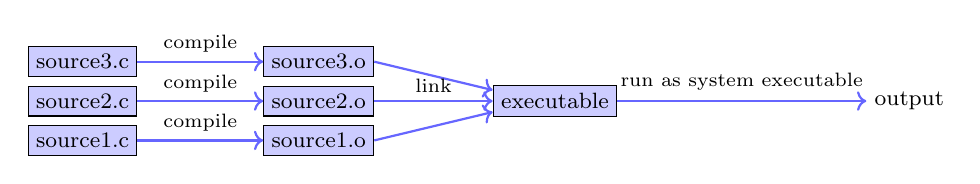
\begin{tikzpicture}
    {\footnotesize
      \node(s3) at (0,1.0) [fill=blue!20,draw] {source3.c};
      \node(s2) at (0,0.5) [fill=blue!20,draw] {source2.c};
      \node(s1) at (0,0.0) [fill=blue!20,draw] {source1.c};
      
      \node(o3) at (3,1.0) [fill=blue!20,draw] {source3.o};
      \node(o2) at (3,0.5) [fill=blue!20,draw] {source2.o};
      \node(o1) at (3,0.0) [fill=blue!20,draw] {source1.o};
      
      \node(x) at (6,0.5) [fill=blue!20,draw]  {executable};

      \node(out) at (10.5,0.5) {output};

      \draw (s3.east) edge[->, blue!60, thick] node[above,black]{\scriptsize compile} (o3.west);
      \draw (s2.east) edge[->, blue!60, thick] node[above,black]{\scriptsize compile} (o2.west);
      \draw (s1.east) edge[->, blue!60, thick] node[above,black]{\scriptsize compile} (o1.west);

      \draw (o3.east) edge[->, blue!60, thick]  (x.170); 
      \draw (o2.east) edge[->, blue!60, thick] node[above,black]{\scriptsize link} (x.180); }
    \draw (o1.east) edge[->, blue!60, thick]  (x.190);

    \draw (x.east) edge[->, blue!60, thick]  node[above,black]{\scriptsize run as system executable} (out.west);
  \end{tikzpicture}

\end{frame}


\only<beamer>{
  \begin{frame}{Compiling\ldots{}}

    \begin{center}
      \includegraphics[width=0.8\textwidth]{pic/compiling}
    \end{center}

    \ldots{} from xkcd

  \end{frame}
}

\begin{frame}{Compiled languages in Scientific Computing}

  \begin{itemize}
    \tightlist
  \item
    Fortran: FORmula TRANslator (1957)

    \begin{itemize}
      \tightlist
    \item
      Fortran4: really dead
    \item
      Fortran77: large number of legacy libs: BLAS, LAPACK, ARPACK
      \ldots{}
    \item
      Fortran90, Fortran2003, Fortran 2008

      \begin{itemize}
        \tightlist
      \item
        Catch up with features of C/C++
        (structures,allocation,classes,inheritance, C/C++ library calls)
      \item
        Lost momentum among new programmers
      \item
        Hard to integrate with C/C++
      \item
        In many aspects very well adapted to numerical computing
      \item
        Well designed multidimensional arrays
      \end{itemize}
    \end{itemize}
  \item
    C: General purpose language

    \begin{itemize}
      \tightlist
    \item
      K\&R C (1978) weak type checking
    \item
      ANSI C (1989) strong type checking
    \item
      Had structures and allocation early on
    \item
      Numerical methods support via libraries
    \item
      Fortran library calls possible
    \end{itemize}
  \item
    C++: \emph{The} powerful object oriented language

    \begin{itemize}
      \tightlist
    \item
      Superset of C (in a first approximation)
    \item
      Classes, inheritance, overloading, templates (generic programming)
    \item
      C++11: $\approx 2011$ Quantum leap: smart pointers, threads, lambdas, initializer
      lists in standard
    \item Since then: C++14, C++17, C++20
    \item
      With great power comes the possibility of great failure\ldots{}
    \end{itemize}
  \end{itemize}

\end{frame}

\begin{frame}[fragile]{High level scripting languages}

  \begin{itemize}
    \tightlist
  \item
    Algorithm description using mix of mathematical formulas and
    statements inspired by human language
  \item 
    Simpler syntax, less "boiler plate"
  \end{itemize}

  \begin{pythoncode}
    print("Hello world")
  \end{pythoncode}

  \begin{itemize}
    \tightlist
  \item
    Need intepreter in order to be executed
  \item
    Very far away from CPU \(~\Rightarrow\) usually significantly slower
    compared to compiled languages
  \item
    Matlab, Python, Lua, perl, R, Java, javascript
  \item
    Less strict type checking, powerful introspection
    capabilities
  \item
    Immediate workflow: ``just run''

    \begin{itemize}
      \tightlist
    \item
      in fact: first compiled to \emph{bytecode} which can be interpreted
      more efficiently
    \end{itemize}
  \end{itemize}

  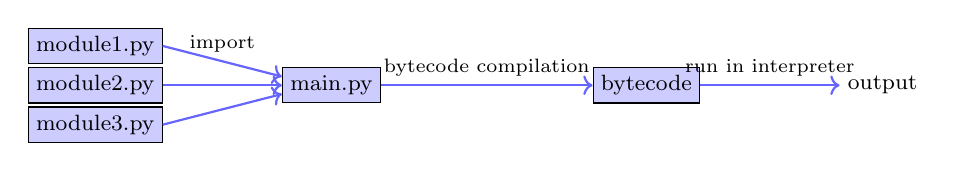
\begin{tikzpicture}
    {\footnotesize
      \node(s3) at (3,1.0) [fill=blue!20,draw] {module1.py};
      \node(s2) at (3,0.5) [fill=blue!20,draw] {module2.py};
      \node(s1) at (3,0.0) [fill=blue!20,draw] {module3.py};

      \node(x) at (6,0.5) [fill=blue!20,draw]  {main.py};


      \node(b) at (10,0.5) [fill=blue!20,draw]  {bytecode};

      \node(out) at (13,0.5) {output};


      \draw (s3.east) edge[->, blue!60, thick] node[above,black]{\scriptsize import}  (x.170); 
      \draw (s2.east) edge[->, blue!60, thick] (x.180); 
    \draw (s1.east) edge[->, blue!60, thick]  (x.190);
    \draw (x.east) edge[->, blue!60, thick]  node[above,black]{\scriptsize bytecode compilation} (b.west);

    \draw (b.east) edge[->, blue!60, thick]  node[above,black]{\scriptsize run in interpreter} (out.west);
    }
  \end{tikzpicture}

\end{frame}

\begin{frame}{JIT based languages}

  \begin{itemize}
    \tightlist
  \item
    Most interpreted language first compile to
    bytecode wich then is run in the interpreter and not on the processor $\Rightarrow$ perfomance bottleneck,
    \begin{itemize}
      \tightlist
    \item  remedy: use compiled language  for performance critical parts
    \item  ``two language problem'', additional work for interface code
    \end{itemize}
  \item Better: Just In Time compiler (JIT): compile to machine code ``on the fly''
    \begin{itemize}
      \tightlist
    \item
      V8 \(~\to\) javascript
    \item
      LuaJIT, Java, Smalltalk
    \item   LLVM    \(~\to\)   \textbf{Julia} (v1.0 since August, 2018)
    \item
      LLVM Compiler infrastructure \(~\to\) Python/NUMBA
    \end{itemize}
  \item
    Drawback over compiled languages: compilation delay at every start,
    can be mediated by caching
  \item
    Advantage over compiled languages: simpler syntax, \emph{tracing} JIT,
    i.e.~optimization at runtime
\end{itemize}
\vfill

  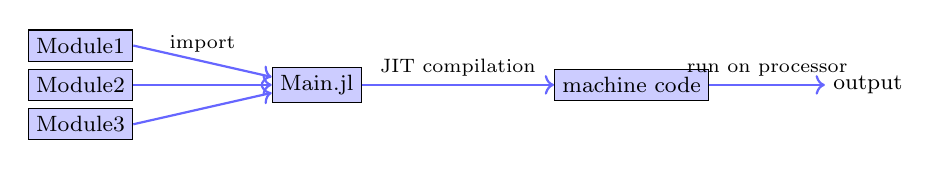
\begin{tikzpicture}
    {\footnotesize
      \node(s3) at (3,1.0) [fill=blue!20,draw] {Module1};
      \node(s2) at (3,0.5) [fill=blue!20,draw] {Module2};
      \node(s1) at (3,0.0) [fill=blue!20,draw] {Module3};

      \node(x) at (6,0.5) [fill=blue!20,draw]  {Main.jl};


      \node(b) at (10,0.5) [fill=blue!20,draw]  {machine code};

      \node(out) at (13,0.5) {output};


      \draw (s3.east) edge[->, blue!60, thick] node[above,black]{\scriptsize import}  (x.170); 
      \draw (s2.east) edge[->, blue!60, thick] (x.180); 
    \draw (s1.east) edge[->, blue!60, thick]  (x.190);
    \draw (x.east) edge[->, blue!60, thick]  node[above,black]{\scriptsize JIT compilation} (b.west);

    \draw (b.east) edge[->, blue!60, thick]  node[above,black]{\scriptsize run on processor} (out.west);
    }
  \end{tikzpicture}


\end{frame}


\begin{frame}\frametitle{Julia History \& Resources}
  \begin{columns}
    \begin{column}{0.6\textwidth}
  \begin{itemize}
  \item 2009-02:  V0.1 Development started in 2009 at MIT (S. Bezanson, S. Karpinski, V. Shah, A. Edelman)
    
  \item    2012: V0.1
    
  \item 2016-10: V0.5 experimental threading support
  \item 2017-02: SIAM Review: Julia - A Fresh Approach to Numerical Computing
  \item 2018-08: \textbf{V1.0}
  \item 2018 Wilkinson Prize for numerical software
  \end{itemize}

    \end{column}
    \begin{column}{0.4\textwidth}
      \begin{center}
        \includegraphics[width=0.5\textwidth]{julia}
        \includegraphics[width=\textwidth]{julia-langauge-developers-mit-00_0}      
      \end{center}
    \end{column}
  \end{columns}

  \vfill
  \begin{itemize}
  \item Homepage incl. download link: \url{https://julialang.org/}
  \item Wikibook: \url{https://en.wikibooks.org/wiki/Introducing_Julia}
  \item TU Berlin Jupyter server \url{https://www-pool.math.tu-berlin.de/jupyter}: you will
    be able to user your UNIX pool account
  \end{itemize}


\end{frame}
%%%%%%%%%%%%%%%%%%%%%%%%%%%%%%%%%%%%%%%%%%%%%%%%%%%%%%%%%%%%%%%%%%%%%%%%%%%%%% 


%%%%%%%%%%%%%%%%%%%%%%%%%%%%%%%%%%%%%%%%%%%%%%%%%%%%%%%%%%%%%%%%%%%%%%%%%%%%%% 
\begin{frame}\frametitle{Julia - a first characterization}
``\textbf{Like matlab, but faster}''

``\textbf{Like matlab, but open source}''

``\textbf{Like python + numpy, but faster and counting from 1}''

  \begin{itemize}
  \item Main purpose: performant numerics 
  \item Multidimensional arrays as first class objects\\
    (like Fortran, Matlab; unlike C++, Swift, Rust, Go $\dots$)
  \item  Array indices counting from 1\\ (like Fortran, Matlab; unlike C++, python) - but it seems this becomes
    more flexible
  \item Array slicing etc.
  \item Extensive library of standard functions, linear algebra operations
  \item Package ecosystem
  \end{itemize}
\end{frame}
%%%%%%%%%%%%%%%%%%%%%%%%%%%%%%%%%%%%%%%%%%%%%%%%%%%%%%%%%%%%%%%%%%%%%%%%%%%%%% 

%%%%%%%%%%%%%%%%%%%%%%%%%%%%%%%%%%%%%%%%%%%%%%%%%%%%%%%%%%%%%%%%%%%%%%%%%%%%%% 
\begin{frame}\frametitle{$\dots$ there is more to the picture}
  \begin{itemize}
  \item Developed from scratch using modern knowledge in language development
  \item Strongly typed $\Rightarrow$ JIT compilation to performant code
  \item Multiple dispatch: all functions are essentialy templates
  \item Parallelization: SIMD, threading, distributed  memory
  \item Reflexive: one can loop over struct elements
  \item Module system, module precompilation
  \item REPL (Read-Eval-Print-Loop)
    
  \item Ecosystem:
    \begin{itemize}
    \item Package manager with github integration
    \item Foreign function interface to C, Fortran, wrapper methods for  C++
    \item PyCall.jl: loading of python modules via reflexive proxy objects (e.g. plotting)
    \item Intrinsic tools for documentation, profiling, testing
    \item Code inspection of LLVM and native assembler codes
    \item IDE integration e.g. via atom editor (Juno)
    \item Jupyter notebooks
    \end{itemize}
  \end{itemize}
\end{frame}
%%%%%%%%%%%%%%%%%%%%%%%%%%%%%%%%%%%%%%%%%%%%%%%%%%%%%%%%%%%%%%%%%%%%%%%%%%%%%% 



%%% Local Variables:
%%% mode: latex
%%% TeX-master: "l01-intro"
%%% End:

\end{document}

